\section{Viivaintegraalit} \label{viivaintegraalit}
\alku
\index{viivaintegraali|vahv}

Tässä luvussa tarkastellaan integraaleja muotoa
\[
I(f,S,\mu)=\int_S f\,d\mu,
\]
missä $S\subset\R^2$ tai $S\subset\R^3$ on (tason tai avaruuden) \kor{käyrä} ja $\mu$ on käyrään
liitettävä \kor{kaarenpituusmitta}. Tällaisia integraaleja sanotaan \kor{viivaintegraaleiksi}
(tai käyräintegraaleiksi). Kaarenpituusmitta pitkin suoraa on tavallinen Jordanin pituusmitta. 
Tasokäyrän (kaaren) $S:\,y=f(x)\ \ja\ x\in[a,b]$ tapauksessa kaarenpituusmitta
on määritelty aiemmin (Luku \ref{kaarenpituus}) ja tulkittu myös integraalin avulla
(Luku \ref{pinta-ala ja kaarenpituus}). Seuraavassa yleistetään tämä käsite ja tutkitaan, miten 
viivaintegraaleja --- ja itse kaarenpituusmittoja --- käytännössä lasketaan.

Otetaan sama lähtökohta kuin Luvussa \ref{parametriset käyrät}, eli oletetaan käyrä $S$ 
parametrisoiduksi reaalimuuttujan $t$ avulla välillä $[a,b]$. Tällöin esimerkiksi avaruuskäyrä
on määritelty $\R^3$:n (tai $E^3$:n) pistejoukkona
\[
S=\{(x,y,z) \ | \ x=x(t), \ y=y(t), \ z=z(t), \ t\in [a,b]\}.
\]
Funktiot $x(t)$, $y(t)$, $z(t)$ (tasokäyrän tapauksessa $x(t)$, $y(t)$) oletetaan jatkossa 
ainakin jatkuviksi välillä $[a,b]$, jolloin käyrässä ei ole 'katkoksia'. Funktioiden
säännöllisyysoletuksia lisätään jatkossa tarpeen mukaan.\footnote[2]{Huomautettakoon, että 
mikäli funktiot $x(t)$, $y(t)$ ja $z(t)$ ovat pelkästään jatkuvia, ei käyrän $S$ 'ulkonäöstä'
voi tehdä pitkälle meneviä johtopäätöksiä. Esimerkiksi on konstruoitavissa välillä $[0,1]$ 
jatkuvat funktiot $x(t)$ ja $y(t)$ siten, että
$S=\{(x(t),y(t)) \ | \ t\in [0,1]\}=[0,1]\times [0,1]$ (!).
Ensimmäisenä tällaisen 'täyteiskäyrän' kostruoi \hist{G. Peano} vuonna 1890. 
\index{Peanon käyrä|av}} 

Jos käyrän parametrisointi $t\in[a,b]\mapsto\vec r\,(t)$ on injektio puoliavoimella välillä
\index{yksinkertainen!c@käyrä, kaari} \index{Jordan-käyrä} \index{suljettu käyrä}%
$[a,b)$, niin kyseessä on \kor{yksinkertainen käyrä} eli \kor{Jordan-käyrä}. Jos lisäksi
$\vec r\,(a)=\vec r\,(b)$, niin käyrä on \kor{suljettu}.
\begin{figure}[H]
\begin{center}
\input{kuvat/kuvaUint-30.pstex_t}
\end{center}
\end{figure}
Jatkossa esitettävässä laskutekniikassa käyrän parametrisoinnilta edellytetään vain riittävä
säännöllisyys. Käyrän ei siis tarvitse olla Jordan-käyrä vaan se voi olla itseään leikkaava tai
jopa itsensä päälle kiertyvä.
\begin{Exa}
Yksikköympyrä tai sen kaari voidaan parametrisoida muodossa
\[
S=\{\,(x,y)\in\R^2 \ | \ x=\cos t, \ y=\sin t, \ t\in [a,b]\,\}.
\]
Tämä on Jordan-käyrä (ympyräkaari), jos $b-a<2\pi$, ja suljettu Jordan-käyrä, jos $b-a=2\pi$.
Yleisemmin kyseessä on parametrinen käyrä, jonka voi tulkita esim.\ edustavan tasaista
ympyräliikettä (aikaparametrisointi). \loppu
\end{Exa}
\begin{Exa} Ruuviviiva on avaruuden (ei-suljettu) Jordan-käyrä muotoa
\[
S=\{\,(x,y,z)\in\R^3 \ | \ x=R\cos t, \ y=R\sin t, \ z=ct, \ t\in [a,b]\,\},
\]
missä $R>0$ ja $c \neq 0$. \loppu
\end{Exa}

\subsection*{Kaarenpituusmitta}
\index{kaarenpituusmitta|vahv}

Yleistetään aluksi kaarenpituusmitan käsite Luvusta \ref{kaarenpituus} parametriselle 
avaruuskäyrälle $S = \{(x(t),y(t),z(t)) \mid t \in [a,b]\}$. (Tasokäyrä tulee käsitellyksi
erikoistapauksena $z(t)=0$.) Olkoon $\{t_k, \ k=0,\ldots n\}$ välin $[a,b]$ jako 
($a=t_0<t_1<\ldots<t_n=b,\ n\in\N$), olkoon 
$\mathcal{P}=\{P_k=(x(t_k),y(t_k),z(t_k)),\ k=0,\ldots,n\}$, ja olkoon edelleen 
$S_{\mathcal{P}}$ janoista $P_{k-1}P_k$, $k=1\ldots n\,$ koostuva murtoviiva. Tällöin jos
kaarenpituusmitalle oletetaan perusaksioomat
\begin{itemize}
\item[-] aksiooma 1: $\quad$ janan $AB$ $\text{mitta}=\abs{\overrightarrow{AB}}$,
\item[-] aksiooma 2: $\quad$ mitan additiivisuus murtoviivalla,
\end{itemize}
niin $S_{\mathcal{P}}$:n pituusmitta on
\[
\mu(S_{\mathcal{P}})=\sum_{k=1}^n\abs{\vec r\,(t_k)-\vec r\,(t_{k-1})}.
\]
Kuten aiemmin Luvussa \ref{kaarenpituus}, käyrän $S$ mitta määritellään tällöin
\[
\mu(S)=\sup_{\mathcal{P}} \mu(S_{\mathcal{P}}).
\]
Mitta on määritelty täsmälleen kun reaalilukujoukko $\{\mu(S_{\mathcal{P}})\}$ on rajoitettu,
\index{suoristuva (käyrä)}%
eli $S$ on mitallinen eli \kor{suoristuva} täsmälleen tällä ehdolla.

Ym.\ määritelmästä nähdään, että kaarenpituusmitta muistuttaa Jordan-mittoja sikäli, että 
perusaksioomissa tarvitaan ainoastaan yksinkertaisen perusjoukon (tässä janan) mitta ja 
additiivisuusperiaate. Jordan-mittojen konstruktiota muistuttaa myös kaarenpituuden 
määrittelyssä käytetty approksimaatioperiaate, jonka mukaan käyrää approksimoidaan 
perusjoukkojen äärellisillä yhdistelmillä. 

\subsection*{Kaarenpituusparametrisaatio}
\index{kaarenpituusparametrisaatio|vahv}

Olkoon $S$ suoristuva Jordan-käyrä. Tällöin jos $S(t)$, $t\in [a,b]$ on käyrän $S$ osa, joka
vastaa parametrin arvoja välillä $[a,t]$, niin kaarenpituusmitan määritelmästä ja kuvauksen
$t\mapsto\vec r(t)$ oletetusta injektiivisyydestä seuraa
\[
t_1,t_2\in [a,b] \ \ja \ t_1<t_2 \ 
               \impl \ \mu(S(t_2))-\mu(S(t_1)) \ge \abs{\vec r\,(t_2)-\vec r\,(t_1)} > 0.
\]
\begin{multicols}{2} \raggedcolumns
Näin ollen jos merkitään
\[
s(t)=\mu(S(t)),
\]
niin $s(t)$ on välillä $[a,b]$ aidosti kasvava. 
\begin{figure}[H]
\begin{center}
\import{kuvat/}{kuvaUint-31.pstex_t}
\end{center}
\end{figure}
\end{multicols}
Siis jokaista $s\in [0,\mu(S)]$ vastaa yksikäsitteinen $t\in [a,b]$ siten, että
$\mu(S(t))=s$. Tämän kääntäen yksikäsitteisen vastaavuuden perusteella käyrä $S$ voidaan yhtä
hyvin parametrisoida kaarenpituuden $s$ avulla, eli voidaan kirjoittaa
\[
S=\{P\in E^d \ | \ P\vastaa \vec r=\vec r\,(s), \ 0\leq s\leq\mu(S)\}.
\]
Tätä sanotaan \kor{kaarenpituusparametrisaatioksi}. Sen laskeminen käytännössä on ongelma
sinänsä, eikä siitä olekaan hyötyä viivaintegraaleja käytännössä laskettaessa. Sen sijaan
käyräteorettisten tarkastelujen 'ajatteluparametrisaationa' se on luonnollinen, syystä että
määritelmän perusteella pätee
\[
\abs{\dvr(s)}=1.
\]
Tämän ominaisuuden vuoksi kaarenpituusparametriaatio on 'helpoin' parametrisaatio silloin kun
halutaan tutkia käyrän (parametrisaatiosta riippumattomia) geometrisia ominaisuuksia, vrt.\
Lukujen \ref{derivaatta geometriassa} ja \ref{käyrän kaarevuus} tarkastelut.
Kaarenpituusparametrisaatiota ajatellaan myös yleisessä kaarenpituusmitan merkinnässä
\[
d\mu=ds \quad \text{(kaarenpituusmitta)}.
\]
Tämä merkintä omaksutaan jatkossa.

\pagebreak
\subsection*{Viivaintegraalien laskutekniikka}

Viivaintegraaleja käytännössä laskettaessa lähdetään käyrän tunnetuksi oletetusta 
parametrisaatiosta $t\mapsto\vec r\,(t)$ (joka harvoin on kaarenpituusparametrisaatio) ja 
pyritään tämän avulla 'oikomaan' integraali tavalliseksi määrätyksi integraaliksi yli 
välin $[a,b]$. Tämä tarkoittaa muunnosta
\[
\int_S f\,ds=\int_{[a,b]} g\,d\mu',
\]
missä $g(t)=f(x(t),y(t),z(t))$ ja $\mu'$ on kaarenpituusmitan vastine välillä $[a,b]$. Mitan
$\mu'$ määrittämiseksi menetellään samalla tavoin kuin muuttujan vaihdossa 
(vrt.\ Luku \ref{muuttujan vaihto integraaleissa}). Jos $\Delta S(t)$ on parametriväliä
$[t,t+\Delta t]\subset [a,b]$ vastaava käyrän $S$ osa, niin sikäli kun on määritettävissä
\kor{muuntosuhde} \index{muuntosuhde integraalissa!d@viivaintegraalissa}
\[
J(t)=\lim_{\Delta t\kohti 0^+} \frac{\mu(\Delta S(t))}{\Delta t}\,,
\]
ja lisäksi $J(t)$ on riittävän säännöllinen (esim.\ jatkuva tai paloittain jatkuva), niin
\[
\int_S f\,ds=\int_a^b g(t)J(t)\,dt.
\]
Viivaintegraali on näin palautettu tavalliseksi määrätyksi integraaliksi Jordan-mitan suhteen.

Muuntosuhteen $J(t)$ määräämiseksi oletetaan, että $x(t)$, $y(t)$ ja $z(t)$ ovat jatkuvasti 
derivoituvia välillä $[a,b]$. (Oletus on hiukan lievennettävissä, ks.\ kommentit jäljempänä). 
Olkoon $\Delta S$ käyrän osa välillä $[t,t+\Delta t] \subset [a,b]$ ($\Delta t>0$) ja olkoon
$\{t_j,\ j=0 \ldots n\}$ välin $[t,t+\Delta t]$ jako, ts.\ 
$t=t_0 < t_1 < \ldots < t_n = t+\Delta t$. Tällöin Differentiaalilaskun väliarvolauseen mukaan
\[
x(t_j)-x(t_{j-1})=x'(\xi_j)(t_j-t_{j-1}),\quad \xi_j\in (t_{j-1},t_j).
\]
Koska $x'$ on jatkuva välillä $[a,b]$ ja $\,\xi_j\in[t,t+\Delta t]$, niin tässä
\[
x'(\xi_j) = x'(t) + \ord{1}, \quad \text{kun}\ \Delta t \kohti 0. 
\]
[Tässä nojataan jatkuvuuden syvällisempään logiikkaan (tasaiseen jatkuvuuteen), vrt.\ vastaava
päättely Luvussa \ref{muuttujan vaihto integraaleissa}.] Arvioimalla samalla tavoin
$y(t_j)-y(t_{j-1})$ ja $z(t_j)-z(t_{j-1})$ päätellään, että
\vspace{1mm}
\begin{align*}
&\sqrt{[x(t_j)-x(t_{j-1})]^2+[y(t_j)-y(t_{j-1})]^2+[z(t_j)-z(t_{j-1})]^2} \\[1mm]
&\quad = \sqrt{[x'(t)]^2+[y'(t)]^2 + [z'(t)]^2}\,(t_j-t_{j-1}) 
                                   + \ord{1}(t_j-t_{j-1}), \quad \text{kun}\ \Delta t \kohti 0.
\end{align*}
\vspace{1mm}
Summaamalla yli $j$:n ja käyttämällä kaarenpituuden määritelmää seuraa
\[
\mu(\Delta S)=\abs{\dvr(t)}\Delta t+\ord{\Delta t}, \quad \text{kun}\ \Delta t \kohti 0.
\]
Muuntosuhteen määritelmän nojalla on $J(t)=|\dvr(t)|$. Siis kaarenpituusmitan muunnoskaava 
avaruuskäyrälle on
\[
ds = \abs{\dvr(t)}\,dt = \sqrt{[x'(t)]^2+[y'(t)]^2+[z'(t)]^2}\,dt,
\]
ja viivaintegraalille on saatu laskukaava
\begin{equation} \label{viivaintegraalin kaava}
\boxed{\quad \int_S f\,ds=\int_a^b g(t)\abs{\dvr(t)}\,dt, \quad 
                     g(t)=f(\vec r\,(t)). \quad} \tag{$\star$}
\end{equation}
Kaava on pätevä hieman heikomminkin kuin oletetuin edellytyksin. Esimerkiksi seuraavat oletukset
ovat yhdessä riittävät:
\begin{itemize}
\item[(i)]   $x(t)$, $y(t)$, $z(t)$ ovat jatkuvia välillä $[a,b]$.
\item[(ii)]  $x'(t)$, $y'(t)$ $z'(t)$ ovat olemassa ja jatkuvia avoimilla väleillä 
             $(c_{i-1},c_i)$, $i=1\ldots m$, missä $a=c_0<c_1<\ldots<c_m=b$ $(m\in\N)$.
\item[(iii)] $g(t)\abs{\dvr(t)}$ on (laajennetussa mielessä) Riemann-integroituva välillä
             $[a,b]$.
\end{itemize}
Sovelluksissa ei näitä lievennyksiä pitemmälle ole juuri tarvetta mennä.

Jos kaavassa \eqref{viivaintegraalin kaava} asetetaan $f=1$ $(\impl g=1)$, on tuloksena
kaarenpituuden laskukaava
\[
\boxed{\kehys\quad \mu(S)=\int_a^b \abs{\dvr(t)}\,dt. \quad}
\]
Huomattakoon, että jos käytetään kaarenpituusparametrisaatiota $(t=s)$, niin $a=0$, $b=\mu(S)$
ja $\abs{\dvr(s)}=1$, jolloin kaava saa muodon
\[
\mu(S)=\int_0^{\mu(S)}ds=\sijoitus{0}{\mu(S)} s=\mu(S).
\]
Tämä on luonnollisesti vain tautologia, josta ei ole käytännön hyötyä kaarenpituuden
laskemisessa.
\begin{multicols}{2}
\begin{Exa}
Ohuesta, tasapaksusta ja homogeenisesta langasta valmistettu kierrejousi on avaruuskäyrä 
$x=R\cos t$, $y=R\sin t$, $z=Ht/(12\pi)$,  $0 \le t \le 12\pi$. Laske a) jousen pituus, 
b) hitausmomentti suoran $x=R$, $y=0$ suhteen, kun jousen massa $=m$.
\begin{figure}[H]
\begin{center}
\import{kuvat/}{kuvaUint-33.pstex_t}
\end{center}
\end{figure}
\end{Exa}
\end{multicols}
\ratk a)
\begin{align*}
\mu(S) &= \int_0^{12\pi} \sqrt{[x'(t)]^2+[y'(t)]^2+[z'(t)]^2}\,dt \\
       &= \int_0^{12\pi} \sqrt{R^2+\left(\frac{H}{12\pi}\right)^2}\,dt \\[2mm]
       &= \underline{\underline{\sqrt{(12\pi R)^2+H^2}}}\,.
\end{align*}

b) Olkoon langan massatiheys pituusyksikköä kohti $=\rho_0$, jolloin a-kohdan mukaan 
$m = \rho_0\sqrt{(12\pi R)^2+H^2}$. Hitausmomentti suoran $S:\ x=R,\ y=0$ suhteen on
\begin{align*}
I_S &= \int_S \left[(x-R)^2+y^2\right]\,\rho_0\,ds \\
    &= \int_0^{12\pi} \rho_0 R^2 \left[(1-\cos t)^2 + \sin^2 t\right]
                       \sqrt{R^2+\left(\frac{H}{12\pi}\right)^2}\,dt \\
    &= \frac{mR^2}{12\pi}\int_0^{12\pi}(2-2\cos t)\,dt \\[2mm]
    &= \underline{\underline{2mR^2}}.
\end{align*}

Tähän tulokseen olisi voitu tulla ilman integrointiakin: Koska langan koko massa on
vakioetäisyydellä $R\,$ $z$-akselista, niin hitausmomentti $z$-akselin suhteen on
$I_z=mR^2$, jolloin Steinerin säännöstä (ks.\ edellinen luku) seuraa $I_S=mR^2+mR^2=2mR^2$.
\loppu 

\subsection*{Tasokäyrät}

Tasokäyrän tapauksessa on $\,\abs{\dvr(t)}=\sqrt{[x'(t)]^2+[y'(t)]^2}$.
Jos käyrä on annettu muodossa $y=f(x)$ ja valitaan $t=x$, niin saadaan 
(ennestään tuttu, vrt.\ Luku \ref{pinta-ala ja kaarenpituus}) tulos
$\,\abs{\dvr(x)}=\sqrt{1+[f'(x)]^2}$. Jos taas käyrä on annettu polaarimuodossa
$\,r=f(\varphi)$, niin on luonnollista valita parametriksi $t=\varphi$, jolloin
\begin{align*}
x'(\varphi) &= \frac{d}{d\varphi}[f(\varphi)\cos\varphi]
             = f'(\varphi)\cos\varphi-f(\varphi)\sin\varphi, \\
y'(\varphi) &= \frac{d}{d\varphi}[f(\varphi)\sin\varphi]
             = f'(\varphi)\sin\varphi+f(\varphi)\cos\varphi,
\end{align*}
ja näin ollen
\[
\abs{\dvr(\varphi)}=\sqrt{[x'(\varphi)]^2+[y'(\varphi)]^2}
                   =\sqrt{[f(\varphi)]^2+[f'(\varphi)]^2}.
\]
Laskettaessa viivaintegraaleja tasokäyrien yli voidaan siis käyrän esitysmuodosta riippuen
käyttää mittamuunnoksia
\index{muuntosuhde integraalissa!d@viivaintegraalissa}
\index{kzyyrzy@käyräviivaiset koordinaatistot!d@--integraalit}%
\[ \boxed{
\quad ds=\begin{cases}
\sqrt{[x'(t)]^2+[y'(t)]^2}\,dt &(\,x=x(t), \ y=y(t)\,) \quad\ykehys \\
\sqrt{1+[f'(x)]^2}\,dx &(\,y=f(x)\,) \\
\sqrt{[f(\varphi)]^2+[f'(\varphi)]^2}\,d\varphi &(\,r=f(\varphi)\,) \akehys
\end{cases} } \]
\begin{Exa}
Laske puoliympyrän kaaren $S:\ x^2+y^2=R^2,\ y \ge 0\ $ pituus $\mu(S)$ kolmella eri tavalla.
\end{Exa}
\ratk
(a) \ \, $x=R\cos t$, $\,y=R\sin t$, $\,t\in [0,\pi]$
\[
\impl \mu(S)=\int_0^\pi \sqrt{[x'(t)]^2+[y'(t)]^2}\,dt
            =\int_0^\pi R\,dt=\underline{\underline{\pi R}}.
\]
(b) \ \, $y=\sqrt{R^2-x^2}=f(x)$, $\,x\in [-R,R]$
\begin{align*}
\impl \ \mu(S) &= \int_{-R}^R \sqrt{1+[f'(x)]^2}\,dx=\int_{-R}^R \frac{R}{\sqrt{R^2-x^2}}\,dx \\
               &= \int_{-\pi/2}^{\pi/2} R\,dt
                = \underline{\underline{\pi R}}. \qquad [\,\text{sijoitus}\ x=R\sin t\,]
\end{align*}
(c) \ \, $r=R=f(\varphi)$, $\,\varphi\in [0,\pi]$
\[
\impl \ \mu(S)=\int_0^\pi \sqrt{[f(\varphi)]^2+[f'(\varphi)]^2}\,d\varphi
              =\int_0^\pi R\,d\varphi=\underline{\underline{\pi R}}. \loppu
\]

\begin{multicols}{2}
\begin{Exa}
Logaritmisen spiraalin $r=e^{-\varphi}$ kaarenpituus välillä $\varphi\in [0,\infty)$ on
\begin{align*}
\mu(S) &= \int_0^\infty \sqrt{[f(\varphi)]^2+[f'(\varphi)]^2}\,d\varphi \\
       &= \int_0^\infty \sqrt{2}\,e^{-\varphi}\,d\varphi\
        =\ \underline{\underline{\sqrt{2}}}. \loppu
\end{align*}
\begin{figure}[H]
\begin{center}
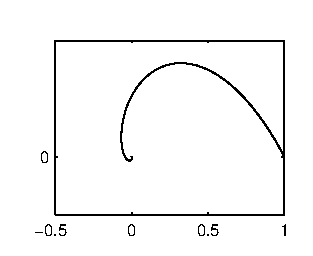
\epsfig{file=kuvat/kuvaUint-32.eps}
\end{center}
\end{figure}
%\end{Exa}
%\end{multicols}
\end{Exa}
\end{multicols}
\begin{Exa}
Laske viivaintegraali $\int_S f\,ds$, kun \ a) $f(x,y)=y$, \ b) $f(x,y)=x$ ja
$S=\{\,(x,y)\in\R^2 \mid y=x^3/3 \ \ja \ x\in [0,1]\,\}$. 
\end{Exa}
\ratk
\begin{align*}
a) \qquad \int_S y\,ds &= \int_0^1 \frac{1}{3}x^3\sqrt{1+x^4}\,dx \\
                       &=\sijoitus{0}{1} \frac{1}{18}(1+x^4)^{3/2}
                        =\underline{\underline{\frac{1}{18}(2\sqrt{2}-1)}}. \\[2mm]
b) \qquad \int_S x\,ds &= \int_0^1 x\sqrt{1+x^4}\,dx \qquad 
                              [\,\text{sijoitus}\ x^2=t, \ x\,dx=\tfrac{1}{2}\,dt\,] \\
                       &=\frac{1}{2}\int_0^1 \sqrt{1+t^2}\,dt \qquad 
                              [\,\text{sijoitus}\ t=\sinh u, \ dt=\cosh u\,du\,] \\
                       &=\frac{1}{2}\int_{0}^{\ln (\sqrt{2}+1)} \cosh^2 u\,du \\
                       &=\frac{1}{8}\int_{0}^{\ln (\sqrt{2}+1)} (e^{2u}+e^{-2u}+2)\,du \\
                       &=\frac{1}{16}\sijoitus{0}{\ln (\sqrt{2}+1)}(e^{2u}-e^{-2u}+4u) 
                        =\underline{\underline{
                         \frac{1}{4}\bigl[\sqrt{2}+\ln(\sqrt{2}+1)\bigr]}}. \loppu
\end{align*}

\Harj
\begin{enumerate}

\item
Rautalanka, jonka pituus $=10\pi$, on taivuteltu noudattamaan pisteestä $(3,0,0)$ lähtien \
a) ruuviviivaa $\,S:\, x=3\cos t,\ y=3\sin t,\ z=4t,\ t \ge 0$, \ b) käyrää
$\,S:\, x=3\cos^2t,\ y=4\sin^2t,\ z=5\sin t\cos t,\ t \ge 0$. Laske langan toinen päätepiste.

\item
Laske viivaintegraali $\int_S f\,ds$ annetuilla $f$ ja $S$\,: \vspace{1mm}\newline
a) \ $f(x,y)=xy, \quad S:\ x=2\cos t,\ y=\sin t,\ t\in[0,\frac{\pi}{2}]$ \newline
b) \ $f(r,\varphi)=r^2\varphi, \quad S:\ r=\varphi,\ \varphi\in[0,4\pi]$ \ (polaarik.) \newline
c) \ $f(x,y,z)=x^2z, \quad S:\ r=1,\ z=\varphi,\ \varphi\in[0,4\pi]$ \ (lieriök.) \newline
d) \ $f(x,y,z)=x^2z^3, \quad S:\ r=1,\ \theta=2\pi/3,\ \varphi\in[0,3\pi]$ \ (pallok.)

\item
Käyrän kaaren $S:\,t\in[a,b]\map\vec r\,(t)$ (matemaattinen) keskiö lasketaan kaavalla
$\vec r_0 = \frac{1}{\mu(S)} \int_S \vec r\,ds$. Sovella kaavaa: \vspace{1mm}\newline
a) \ $\vec r=R\cos t\vec i+R\sin t\vec j,\ t\in[0,\pi]\ $ (puoliympyrä) \newline
b) \ $\vec r=R(t-\sin t)\vec i+R(1-\cos t)\vec j,\ t\in[0,2\pi]\ $ (sykloidin kaari) \newline
c) \ $\vec r=R\cos^3 t\,\vec i+R\sin^3 t\,\vec j,\ t\in[0,\pi/2]\ $ (asteroidin kaari)

\item
Suoran langan pätepisteet ovat $(0,0)$ ja $(2a,0)$ ja langan massatiheys pituusyksikköä kohti
on $\rho(x)=\rho_0(1+x/a)$ ($\rho_0=$ vakio, $a>0$). Lanka taivutetaan noudattamaan origosta
lähtien ympyräviivaa $x^2+y^2=2ay,\ x \ge 0$. Määritä taivutetun langan painopiste.

\item
Lenkkeilijä lähtee pisteestä $(1,0)$ (pituusyksikkö = km) kiertämään pururataa $S: x^2+y^2=1$
vastapäivään. Missä pisteessä lenkkeilijä on tunnin juostuaan, jos hänen juoksuvauhtinsa on \ 
$v(s)=v_0e^{-0.05s}$, missä $v_0=12$ km/h ja $s=$ juostu matka kilometreina?

\item (*)
Esitä seuraavat käyrät kaarenpituusparametrisaation avulla. \vspace{1mm}\newline
a) \ $x=R(t-\sin t),\ y=R(1-\cos t),\ t\in[0,2\pi]$ \newline
b) \ $y=x^2,\ x \ge 0$

\item (*) \index{zzb@\nim!Laskiainen, 3.\ lasku}
(Laskiainen, 3.\ lasku) Näytä, että harjoitustehtävässä
\ref{toisen kertaluvun dy}:\ref{H-dy-3: nopein liuku} lumilautailijan lyhin laskuaika
pisteeseen $P=(a,0)$ ($a>0$) on $t_{min}=\sqrt{2\pi a/g}$.

\item (*)
Lieriöt $L_1: x^2+y^2=R^2$, $L_2: (y-R)^2+z^2=R^2$ ja pallo $K: (x-R)^2+y^2+z^2=R^2$ leikkaavat
toisensa pitkin kolmea avaruuskäyrää. Näytä, että näiden leikkauskäyrien pituudet 
ovat \vspace{1mm}\newline
a) \,\ $\mu(L_1 \cap L_2) = \int_0^{\pi/2} \sqrt{f(\sin t)}\,dt, \quad
                                   f(x)=[1-x^2(1-x)^2]/(2x-x^2)$, \newline
b) \,\ $\mu(L_1 \cap K) = \mu(L_2 \cap K) = \int_{\pi/6}^{\pi/2} \sqrt{g(\sin t)}\,dt, \quad
                                   g(x)=(2x-x^2)/(2x-1)$.

\item (*) \index{zzb@\nim!Kzz@Köysi katolla}
(Köysi katolla) $xy$-tasolle on pystytetty pitkä rakennus, jonka vesikatto on pinnalla
$z = 4-x^2/2$ ja räystäät suorilla $x=\pm 2,\ z=2$.
Rakennuksen yli on heitetty (hyvin taipuisa) köysi siten, että köyden kumpikin pää ulottuu 
$xy$-tasolle. \ a) Mikä on tällaisen köyden minimipituus? \ b) Mikä on köyden
minimipituus sillä lisäehdolla, että köysi tulee räystäiden yli pisteissä $(2, 2, 2)$ ja
$(-2, -2, 2)\,$? \
c) Millaisena tasokäyränä köysi näkyy b-kohdassa, kun sitä katsellaan kaukaa positiivisen
$z$-akselin suunnasta? 

\end{enumerate}
